%
% Quantum Channels
%

\section{Quantum channels} \label{sec:quant_chan} \index{Quantum channels}

\dropcap{L}{ike} classical channels, quantum channels are inevitably subject to errors. These errors could be an intrinsic part of the system, or induced by interaction with the external environment. The \textit{quantum process} formalism provides an elegant mathematical description for all physically realistic error mechanisms \cite{bib:NielsenChuang00, bib:Gilchrist05}. Here we review the quantum process formalism and how it applies to quantum networks. This paves the way for the quantum notion of costs and attributes.

%
% Quantum Processes
%

\subsection{Quantum processes} \index{Quantum processes}

To quantify the operation of nodes and links within our network, we must characterise the evolution they impose upon quantum states passing through them. Quantum processes, also known as \textit{trace-preserving, completely positive maps} (CP-maps) are able to capture all the physical processes relevant to quantum networking, such as: unitary evolution; decoherence; measurement; quantum memory; state preparation; switching; and, indeed entire quantum computations. And they are able to capture physical processes in any degree of freedom, most commonly in the qubit basis, but also, for photons, in the spatio-temporal, photon-number, phase-space, or polarisation degrees of freedom.

Quantum processes are most easily represented using \textit{Kraus operators}\index{Kraus operators}, $\{\hat{K}_i\}$,
\begin{align} \label{eq:kraus_rep}
\mathcal{E}(\hat\rho) = \sum_i \hat{K}_i \hat\rho \hat{K}_i^\dag,
\end{align}
where,
\begin{align}
\sum_i \hat{K}_i^\dag \hat{K}_i = \hat\openone,
\end{align}
for normalisation. Here $\mathcal{E}$ is a super-operator, denoting the action of the process on state $\hat\rho$. This is also referred to as the \textit{operator-sum representation}\index{Kraus operators}. This representation has the elegant interpretation as the probabilistic application of each of the Kraus operators $\hat{K}_i$, with probability,
\begin{align}
p_i = \mathrm{tr}(\hat{K}_i \hat\rho \hat{K}_i^\dag).
\end{align}
In the ideal case, the two types of evolution of interest are unitary evolution, in which case there is only one Kraus operator, \mbox{$\hat{K}_1=\hat{U}$}, and projective measurement, where there is again only one Kraus operator, \mbox{$\hat{K}_1=\ket{m}\bra{m}$}, for measurement outcome $m$.

Mathematically, quantum processes are equivalent to a state jointly undergoing unitary evolution with an external environment that is not observed (i.e traced out),
\begin{align} \label{eq:proc_environment}
\mathcal{E}(\hat\rho_S) = \mathrm{tr}_E (\hat{U}_{S,E} [\hat\rho_S\otimes \ket{0}_E\bra{0}_E] \hat{U}^\dag_{S,E}),
\end{align}
where $S$ denotes the primary system to which the process is applied, and $E$ is an auxiliary environment system, as shown in Fig.~\ref{fig:q_proc}.

\begin{figure}[!htbp]
\begin{align}
\Qcircuit @C=1em @R=1.6em {
    \lstick{\hat\rho_S} & \multigate{1}{{U}_{S,E}} & \qw & \,\,\,\,\,\mathcal{E}(\hat\rho_S) \\
    \lstick{\ket{0}_E} & \ghost{\hat{U}_{S,E}} & \qw & \times \\
} \nonumber
\end{align}
\captionspacefig \caption{Model for the quantum process formalism, as a system state $\hat\rho_S$ undergoing joint unitary evolution with an environment state $\ket{0}_E$, which is subsequently traced out, yielding an arbitrary quantum process $\mathcal{E}(\hat\rho_S)$ acting on the primary system. For the most general possible class of quantum processes to be enabled, the dimension of the environment Hilbert space must grows quadratically with the dimension of the primary Hilbert space.\index{Hilbert space}} \label{fig:q_proc}
\end{figure}

We will require that all our states are normalised,
\begin{align}
\mathrm{tr}(\hat\rho) = 1,
\end{align}
and that our processes are \textit{trace preserving}. That is, they preserve normalisation,
\begin{align}
\mathrm{tr}[\mathcal{E}(\hat\rho)] = 1.
\end{align}

Multiple consecutive processes may be composed using the notation,
\begin{align}
\mathcal{E}_n(\dots \mathcal{E}_2(\mathcal{E}_1(\hat\rho)))=(\mathcal{E}_n \circ \dots \circ \mathcal{E}_2\circ\mathcal{E}_1)(\hat\rho).
\end{align}
In general, processes do not commute, i.e \mbox{$\mathcal{E}_1\circ \mathcal{E}_2 \neq \mathcal{E}_2\circ \mathcal{E}_1$}. Unless unitary, quantum processes are irreversible, meaning that errors accumulate and cannot be overcome without the overhead of some form of quantum error correction (QEC) \cite{bib:Shor95, bib:CalderbankShor96, bib:NielsenChuang00}. The linearity of Eq.~(\ref{eq:kraus_rep}) implies that quantum processes are also linear\index{Linearity},
\begin{align}
	\mathcal{E}(\hat\rho_1+\hat\rho_2) = \mathcal{E}(\hat\rho_1)+\mathcal{E}(\hat\rho_2).
\end{align}

The only limitation faced by the quantum process formalism is that it is described over discrete-time only. To consider continuous-time evolution, \textit{master equations}\index{Master equations} can be used. These represent the continuous-time evolution of a quantum state as a differential equation in time, combining a usual Hamiltonian term as well as decoherence terms,
\begin{align}
\frac{d\hat\rho}{dt} = -\frac{i}{\hbar}[\hat{H},\hat\rho] + \sum_j (2\hat{L}_j\hat\rho\hat{L}_j^\dag - \{\hat{L}_j^\dag\hat{L}_j,\hat\rho\}),
\end{align}
where $\hat{H}$ is the Hamiltonian of the isolated system undergoing coherent evolution, and $\hat{L}_j$ are the \textit{Lindblat operators}\index{Lindblat operators}, capturing the incoherent component of the dynamics (i.e environmental couplings). Here $[\cdot,\cdot]$ and $\{\cdot,\cdot\}$ are the commutator and anti-commutator respectively.

In this work we will only make use of discrete-time quantum processes, since they naturally correspond to the evolution of states between discrete points within a network -- we are typically only interested in the process undergone by a state from one end of a link to another, not the continuous-time dynamics of what takes place within them.

%
% Quantum Process Matrices
%

\subsection{Quantum process matrices} \index{Quantum process matrices}

In general, the Kraus operator representation for quantum processes is not unique -- there may be multiple choices of Kraus operators that implement identical physical processes. But if the representation is not unique, how do we compare different quantum processes? To address this, it is common to choose a `standard' basis for representing quantum processes, such that they may be consistently and fairly compared. This requires choosing a basis which is complete for operations on the Hilbert space acted upon by the process.

For example, for a single qubit, the Pauli operators\index{Pauli!Operators} -- $\hat\sigma_1$ (identity, $\hat\openone$), $\hat\sigma_2$ (bit-flip, $\hat{X}$), $\hat\sigma_3$ (bit-phase-flip, $\hat{Y}$), and $\hat\sigma_4$ (phase-flip, $\hat{Z}$) -- are complete for single-qubit operations ($\mathbb{C}_2$). Therefore by decomposing our Kraus operators into linear combinations of these basis operators we have a standardised representation for single-qubit processes. Formally, for one qubit,
\begin{align} \label{eq:process_matrix}
\mathcal{E}(\hat\rho) = \sum_{i,j=1}^4 \chi_{i,j} \hat{\sigma}_i\hat\rho\,\hat{\sigma}_j^\dag.
\end{align}

The Hermitian matrix $\chi$ is known as the \textit{process matrix}\index{Process matrices}, from which many other metrics of interest may be directly computed (some of which are discussed in Sec.~\ref{sec:quantum_meas_cost}).

Process matrices share many algebraic properties and interpretations in common with density matrices. The diagonal elements can be regarded as the amplitudes associated with applying each of the four Pauli operators, all of which are non-negative, while the off-diagonal elements represent the coherences between them, i.e whether the operations on the diagonal are being applied probabilistically or coherently. For example, a process that simply randomly applies Pauli operators would have a diagonal process matrix in the Pauli basis. But off-diagonal elements would be indicative of applying coherent superpositions of the operators. Like density matrices, the dimensionality of process matrices grows exponentially with the number of qubits in the system being characterised, and for exactly the same conceptual reasons.

For the process to be trace preserving we require,
\begin{align}
\mathrm{tr}(\chi) = 1.
\end{align}
We will typically enforce this constraint on our processes. $\mathrm{tr}(\chi) < 1$ implies non-determinism, i.e the process sometimes fails. 

As an illustrative example of the interpretation of process matrices, in Fig.~\ref{fig:CNOT_proc_matrix} we show the process matrix for the CNOT gate, represented in the Pauli basis. The CNOT operator can be expressed in the Pauli operator basis as,
\begin{align}
\hat{U}_\mathrm{CNOT} = \frac{1}{2}(\hat\openone\otimes \hat\openone + \hat\openone \otimes \hat{X} + \hat{Z}\otimes \hat\openone - \hat{Z}\otimes \hat{X}).
\end{align}
Then, some density operator evolved under the CNOT gate is simply \mbox{$\hat{U}_\mathrm{CNOT}\hat\rho \,\hat{U}_\mathrm{CNOT}^\dag$}. Expanding this out, we obtain a new state comprising 16 terms, each representing the action of some combination of Pauli operators from the left and from the right. The amplitudes of these terms exactly correspond to the 16 non-zero elements of the process matrix shown in Fig.~\ref{fig:CNOT_proc_matrix}.

\begin{figure}[!htbp]
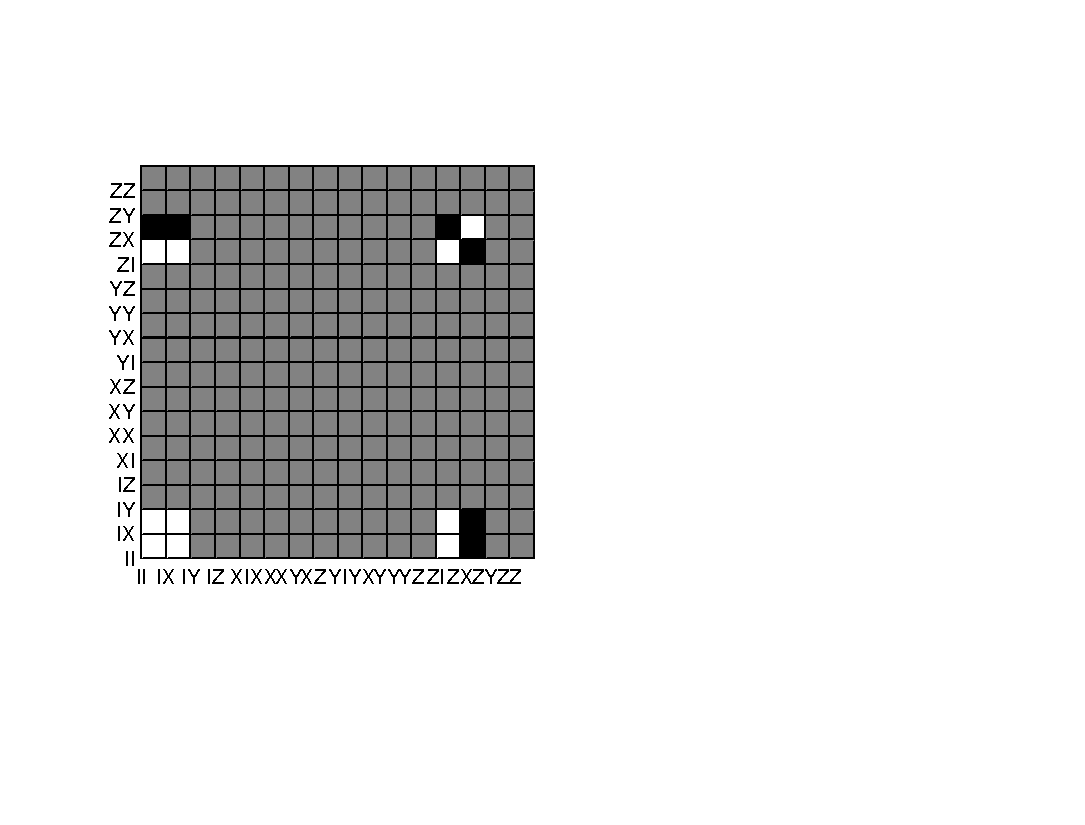
\includegraphics[clip=true, width=0.4\textwidth]{CNOT_process}
\captionspacefig \caption{Process matrix for the CNOT gate, expressed in the Pauli basis. Colour coding: grey=0, white=$1/4$, black=$-1/4$.} \label{fig:CNOT_proc_matrix}
\end{figure}

%
% Quantum Processes in Quantum Networks
%

\subsection{Quantum processes in quantum networks} \label{sec:quant_proc_in} \index{Quantum processes}

Letting $v_i$ represent the $i$th node within a route $R$, the process associated with communication from that node to the next is $\mathcal{E}_{v_i\to v_{i+1}}$. For the same network used previously, Fig.~\ref{fig:example_proc_graph} shows the quantum processes associated with the links in the network. The cumulative process associated with an entire route is therefore,
\begin{align}
\mathcal{E}_R = \mathcal{E}_{{v_{|R|-1}}\to v_{|R|}} \circ \dots \circ \mathcal{E}_{v_2\to v_3} \circ \mathcal{E}_{v_1\to v_2},
\end{align}
where $|R|$ is the number of nodes in $R$, and to simplify notation, all $v_i$ are implicitly over the route $R$.

\begin{figure}[!htbp]
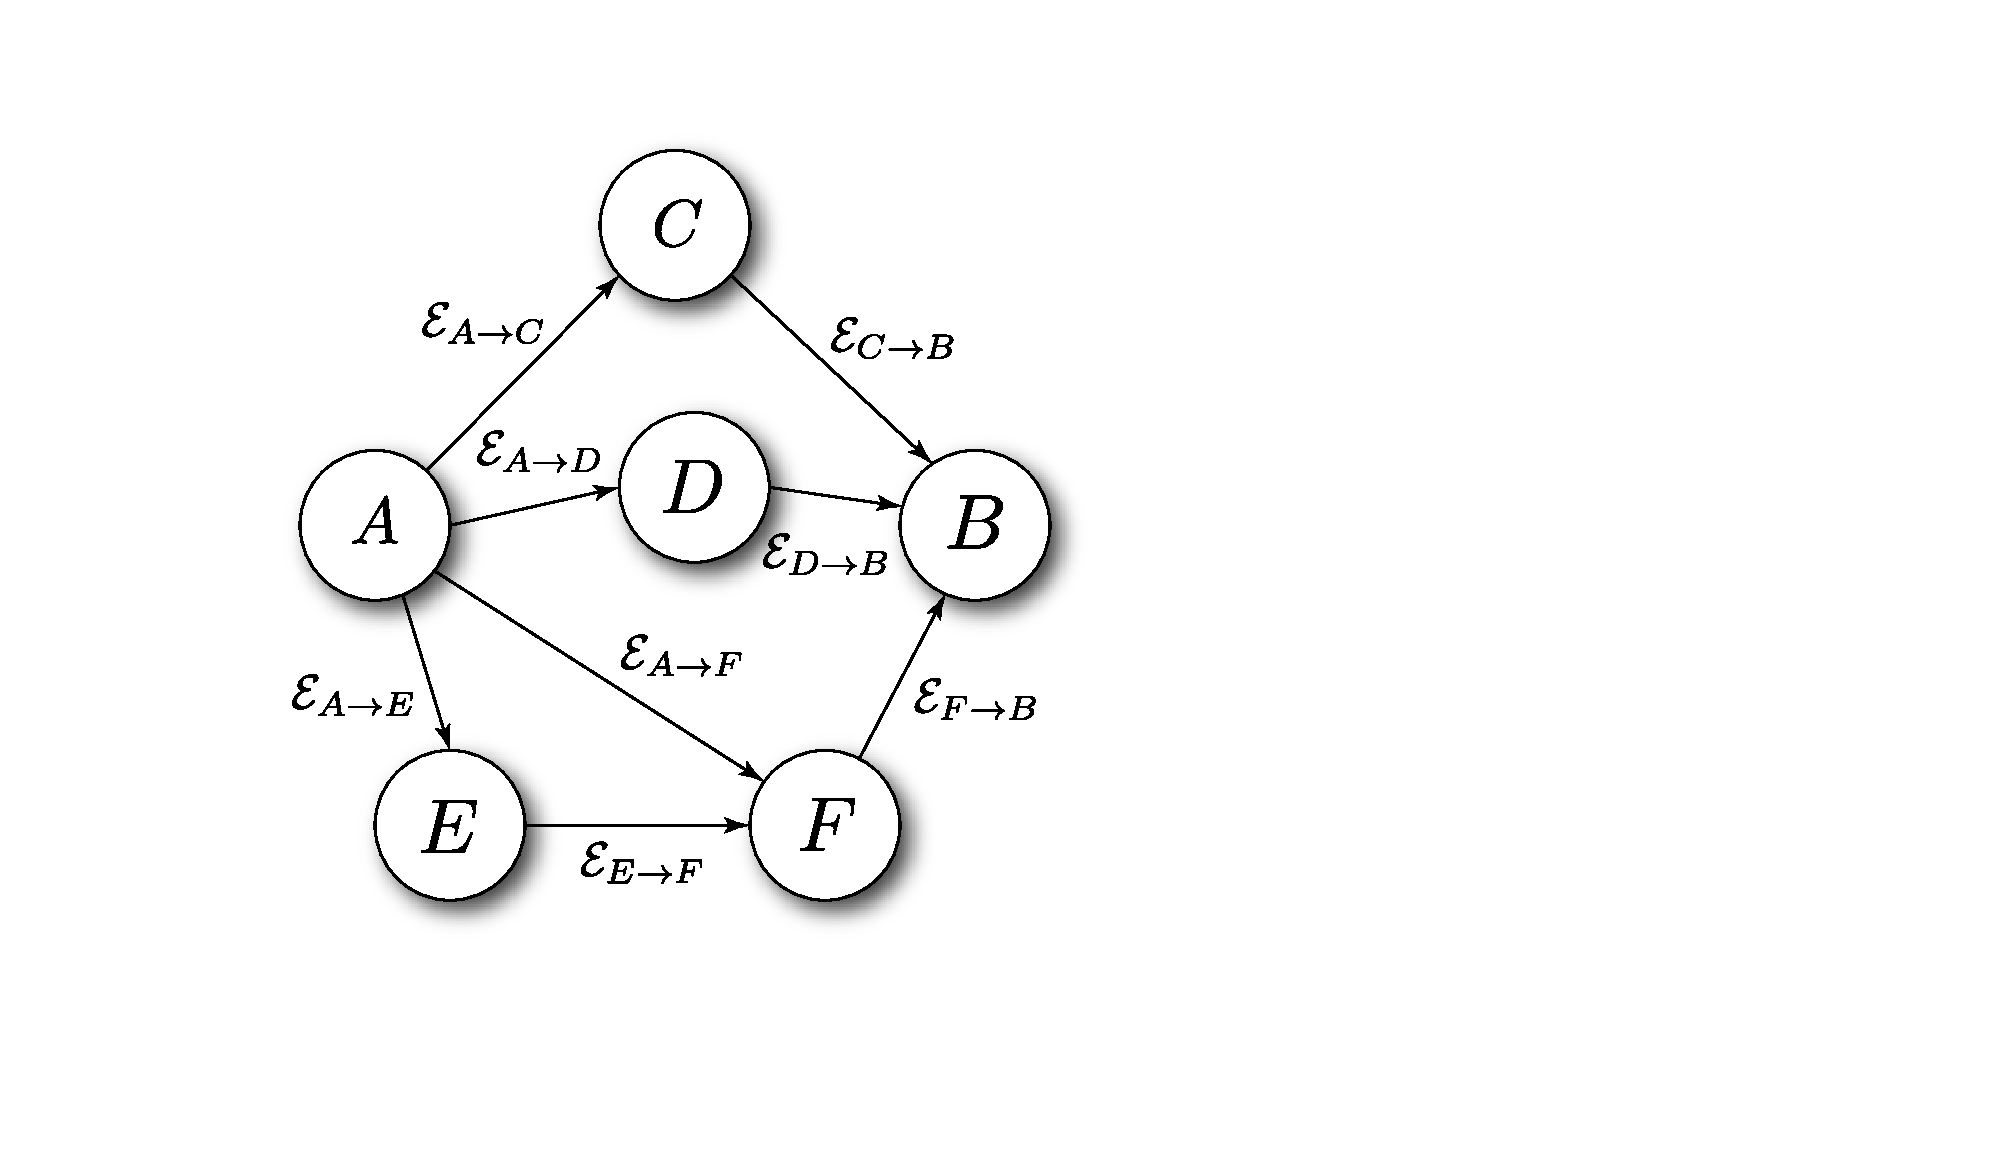
\includegraphics[clip=true, width=0.3\textwidth]{example_graph}
\captionspacefig \caption{The network from Fig.~\ref{fig:example_routes}, with the quantum processes associated with each link. The net process associated with a route is given by the composition of each of the processes over the length of the route. For example, the route \mbox{$R_1=A\to C\to B$} induces the process \mbox{$\mathcal{E}_{R_1} = \mathcal{E}_{C\to B} \circ \mathcal{E}_{A\to C}$}.} \label{fig:example_proc_graph}
\end{figure}

In general, both nodes and links in a quantum network may implement quantum processes. However, for the purposes of compatibility with the graph-theoretic algorithms described in Sec.~\ref{sec:graph_theory}, we will eliminate node processes by merging them into link processes, such that the processes in the network are described entirely by links. This reduction procedure is straightforward, shown in Fig.~\ref{fig:remove_nodes}.

\begin{figure}[!htbp]
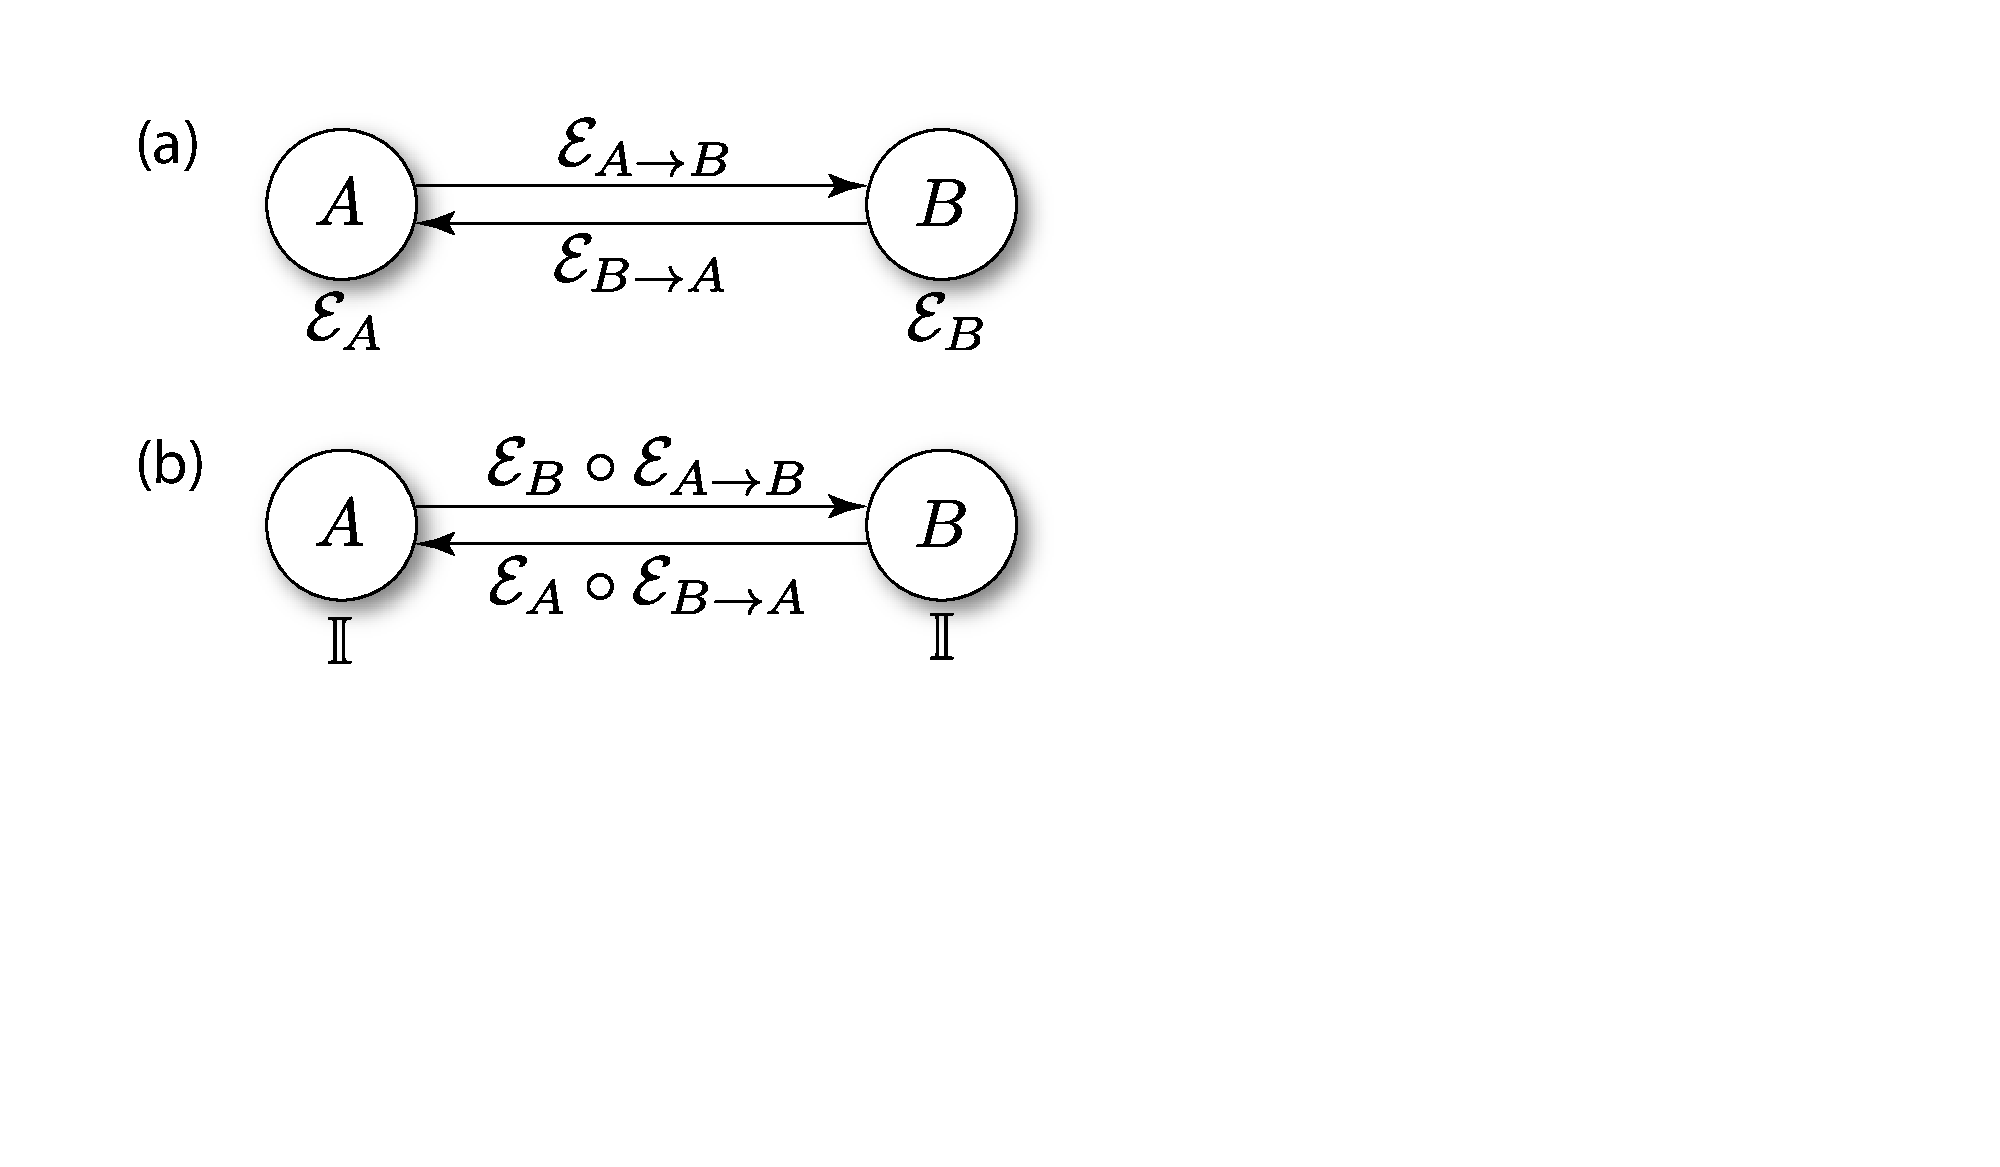
\includegraphics[clip=true, width=0.35\textwidth]{remove_nodes}
\captionspacefig \caption{Removing node processes from network graphs on a trivial network with two nodes, $A$ and $B$. Each node is associated with a quantum process ($\mathcal{E}_A$ and $\mathcal{E}_B$). Similarly, each link is associated with a process ($\mathcal{E}_{A\to B}$ and $\mathcal{E}_{B\to A}$). (a) Representation where the node and link processes are shown explicitly. (b) The node processes are replaced with identity operations by replacing each link process with the composition of the link process and its target node process. Equivalently, the cost of each node process is added to the cost of \textit{every} incoming link and then eliminated. The same may be applied for attributes rather than costs. This procedure requires that all links be directed. If undirected links are present, they may simply be replaced by two directed links, one in each direction, implementing identical quantum processes each way.} \label{fig:remove_nodes}
\end{figure}

%
% Characterising Quantum States & Channels
%

\subsection{Characterising quantum states \& channels} \label{sec:QPT}

Given a link implementing some arbitrary quantum process, it is essential that it can be experimentally determined such that network performance may be characterised. For example, if an optical channel is lossy, what is the loss rate? This is crucial when attempting to choose routing strategies that optimise certain cost metrics.

Treating a link or node as an unknown black box, \textit{quantum process tomography} (QPT) \cite{bib:ChuangNielsen97} is a technique that may be applied to fully characterise the quantum process it implements, reproducing its complete process matrix. QPT has become a standard procedure, demonstrated in numerous architectures, most notably in optics \cite{bib:OBrien04, bib:RohdeGateChar05}.

QPT works in general for processes in any degree of freedom, e.g the qubit degree of freedom. However, it is important to note that full QPT requires statistics across the entire basis over which measurements are defined, which typically grows exponentially with the size of the system. For example, the number of measurement bases required to perform full QPT on $n$ qubits grows exponentially with $n$.

However, often full process characterisation is not necessary. Instead, knowing particular metrics of interest may suffice. Some of the more noteworthy such metrics will be discussed in Sec.~\ref{sec:quantum_meas_cost}. In this instance, much work has been done in the field of \textit{compressed sensing} or \textit{compressed quantum process tomography} \cite{???,compressed_sensing}, in which some process metrics of interest can be experimentally determined using far fewer physical resources (with efficient scaling!) than via a full reconstruction of the process matrix using QPT. As a most trivial example, if the loss associated with a fibre-optic channel is the metric of interest, this can be much more easily determined than by performing full QPT.

On the other hand, however, most quantum channels are designed to accommodate systems with very limited Hilbert space dimensionality per clock-cycle -- e.g a fibre-optic link might transmit just one photon at a time -- in which case there is no exponentiality to be terribly concerned about (QPT of a single-photon channel is trivial).

Importantly, it is often the case that the quantum process associated with a channel will remain constant over time. The efficiency of a length of fibre, for example, does not change. In this instance, characterising the channel need only be performed once in advance, without requiring ongoing dynamic updating. On the other hand, when communicating with satellites in low Earth orbit it is to be expected that the properties of links will be highly dynamic.

We will now explain QPT in the archetypal context of single-qubit channels, which logically generalises to multiple qubits, and can similarly be generalised to non-qubit systems also.

%
% Quantum State Tomography
%

\subsubsection{Quantum state tomography} \index{Quantum state tomography (QST)}

The first stage in QPT is \textit{quantum state tomography} (QST), where the goal is to reconstruct and unknown density matrix via measurements upon multiple copies of the state. QST is based upon the simple observation that the completeness relation\index{Completeness relation} for an arbitrary state can be expressed,
\begin{align}
\hat\rho = \sum_i \mathrm{tr}(\hat{E}_i\hat\rho)\cdot\hat{E}_i,
\end{align}
where $\{\hat{E}_i\}$ forms a complete basis for the Hilbert space of $\hat\rho$. For a single qubit this decomposition is most often performed in the Pauli basis, 
\begin{align}
\hat\rho = \mathrm{tr}(\hat\rho)\cdot\hat\openone + \mathrm{tr}(\hat{X}\hat\rho)\cdot\hat{X} + \mathrm{tr}(\hat{Y}\hat\rho)\cdot\hat{Y} +\mathrm{tr}(\hat{Z}\hat\rho)\cdot\hat{Z}.
\end{align}
Of course, \mbox{$\mathrm{tr}(\hat{E}\hat\rho) = P(\hat{E}|\hat\rho)$} is just the expectation value of the measurement operator $\hat{E}$ when measuring $\hat\rho$. Thus, measuring the expectation values in each of the four Pauli bases reconstructs $\hat\rho$.

This generalises straightforwardly to multi-qubit systems, where we measure all combinations of tensor products of the Pauli operators, the number of which grows exponentially with the number of qubits $n$, as $4^n$. This introduces scalability issues for systems comprising a large number of qubits.

In the case of optical systems, entirely alternate, but equivalent, approaches may be used, such a probing the Wigner function directly using homodyne detection\index{Homodyne detection}.

%
% Quantum Process Tomography
%

\subsubsection{Quantum process tomography} \index{Quantum process tomography (QPT)}

Now to perform QPT we apply the unknown process to a complete basis of input states $\{\hat\rho_i\}$, and perform QST on the output state for each. This yields,
\begin{align}
\mathcal{E}(\hat\rho_j) = \sum_{i} c_{i,j} \hat\rho_i,
\end{align}
where the sum runs over the basis of states. From QST, all the coefficients $c_{i,j}$ may be determined. Next we define the following decomposition for each of the terms in the sum of Eq.~(\ref{eq:process_matrix}),
\begin{align}
\hat{E}_m \hat\rho_j \hat{E}_n^\dag = \sum_k B^{m,n}_{j,k} \hat\rho_k,
\end{align}
where $B$ defines a decomposition in the chosen basis, not dependent on any measurement results. Then we can write,
\begin{align}
\mathcal{E}(\hat\rho_j) &= \sum_{m,n} \chi_{m,n} \hat{E}_m\hat\rho_j\hat{E}_n^\dag \nonumber \\
&= \sum_{m,n} \sum_k \chi_{m,n} B^{m,n}_{j,k} \hat\rho_k.
\end{align}
Because $\hat\rho_k$ form a linearly independent basis, we can write the decomposition,
\begin{align}
c_{j,k} = \sum_{m,n} \chi_{m,n} B_{j,k}^{m,n},
\end{align}
for all \mbox{$j,k$}. From this, standard linear algebra techniques allow an inversion to obtain,
\begin{align}
\chi_{m,n} = \sum_{j,k} (B_{j,k}^{m,n})^{-1} c_{j,k},
\end{align}
thereby obtaining the full process matrix $\chi$, in the chosen basis.